% This is file JFM2esam.tex
% first release v1.0, 20th October 1996
%       release v1.01, 29th October 1996
%       release v1.1, 25th June 1997
%       release v2.0, 27th July 2004
%       release v3.0, 16th July 2014
%   (based on JFMsampl.tex v1.3 for LaTeX2.09)
% Copyright (C) 1996, 1997, 2014 Cambridge University Press

\documentclass{jfm}
%\usepackage{graphicx}
%\usepackage{epstopdf, epsfig}

% My own packages

\usepackage{ dsfont }
\usepackage{amsmath}
\usepackage{hyperref}
%
%% User-defined commands
%
\newcommand{\ddt}[1]{\frac{d #1}{dt}}
%\newcommand{\hmone}[1]{\|#1\|_{H^{-1}}}
\newcommand{\hmone}[1]{\|\nabla^{-1} #1\|_{L^{2}}}
\newcommand{\ltwo}[1]{\|#1\|_{L^{2}}}
%\newcommand{\hone}[1]{\|#1\|_{H^{1}}}
\newcommand{\hone}[1]{\| \nabla #1\|_{L^{2}}}
\newcommand{\htwo}[1]{\|#1\|_{H^{2}}}
\newcommand{\sint}[1]{\int_{D} #1 \, d^{d}\mathbf{x}}
\newcommand{\tint}[1]{\int_{0}^{T} #1 \, dt}
\renewcommand{\vec}[1]{\mathbf{#1}}
\newcommand{\linf}[1]{\| #1 \|_{L^{\infty}}}
\newcommand{\tavg}[1]{\langle  #1 \rangle}
\renewcommand{\u}{\mathbf{u}}
%\newcommand{\ppt}[1]{\frac{\partial #1}{\partial t}}
\newcommand{\ppt}[1]{\partial_{t} #1}
\newcommand{\lap}{\Delta }
\newcommand{\invlap}{\Delta^{-1}}
%\newcommand{\lap}{\nabla^{2}}
%\newcommand{\invlap}{\nabla^{-2}}
\newcommand{\pbrac}[1]{\left( #1 \right)}
\newcommand{\sbrac}[1]{\left[ #1 \right]}
\newtheorem{lemma}{Lemma}
\newtheorem{corollary}{Corollary}

\shorttitle{Diffusion limitations on mixing by incompressible flows}
\shortauthor{C. J. Miles and C. R. Doering}

\title{Diffusion limitations on mixing by incompressible flows}

\author{Christopher J. Miles\aff{1,2,3}
  \corresp{\email{cmiless@umich.edu}}
 \and Charles R. Doering\aff{1,2,3}}

\affiliation{\aff{1}Department of Physics, University of Michigan,
Ann Arbor, MI 48104-1040, USA
\aff{2}Department of Mathematics, University of Michigan,
Ann Arbor, MI 48104-1043, USA
\aff{3}Center for the Study of Complex Systems, University of Michigan,
Ann Arbor, MI 48104-1107, USA}

\begin{document}

\maketitle

\begin{abstract}
An incompressible flow can be an effective mixer of a dye by appropriately advecting the dye to produce small filamentation length scales. It is known that the Batchelor length scale [\cite{Batchelor1959a}] is the theorized lower limit of dye length scales  achievable under turbulent flows. We provide numerical evidence that this limitation may be more general and applies to incompressible flows under mild physical constraints such as fixed enstrophy and energy. We consider local-in-time flow optimization under these constraints with the objective of maximizing mixing rate performance. For enstrophy-bounded optimal flows, we find that the strength of diffusion has no impact on the long-term mixing rate performance. For energy-constrained optimal flows, we find that an increase in the strength of diffusion worsens this performance. We provide analytical lower bounds on mixing rates and length scales achievable under related constraints (pointwise bounded speed and rate-of-strain) by extending the work of \cite{JFM2011} and \cite{Chi-Cheu1996}. 


\end{abstract}

\begin{keywords}
Optimal mixing, incompressible flow, diffusion, Batchelor scale
\end{keywords}

\section{Introduction}

Optimal mixing is important to many areas of science and engineering. A question of interest across these domains is ``How can one stir to enhance the rate of mixing?'' We explore this question and study the impact of molecular diffusion. We address this topic by considering an incompressible flow with mild physical constraints in a periodic box with side length $L$ in $d$ dimensions. We consider a mean-zero tracer concentration field $\theta$ that evolves according to the advection-diffusion equation,
\begin{equation}
	\label{eq:PDE_advection}
	\ppt{\theta}+\mathbf{u}\cdot \nabla \theta=\kappa \lap\theta,
\end{equation}
with initial data $\theta(\mathbf{x},0)=\theta_{0}(\mathbf{x})$, where $\kappa$ is the molecular diffusion coefficient and $\mathbf{u}(\mathbf{x},t)$ is the incompressible ($\nabla\,\cdot\, \vec{u}=0$) flow field. The flow is constrained by enstrophy $\ltwo{\nabla\u} = \Gamma L^{d/2}$ or energy $\ltwo{\u} = UL^{d/2}$ where $\Gamma$ is the root mean square rate-of-strain and $U$ is the root mean square speed. We primarily use the $H^{-1}$ norm or mix-norm throughout to measure homogenization,   

\begin{equation}
\hmone{\theta}=\sqrt{\sint{ |\nabla^{-1} \theta( \vec{x},t)|^2}}=\sqrt{ \sum_{\vec{k}\neq \vec{0}} L^d \frac{|\hat{\theta}_{\vec{k}}(t)|^{2}}{|\vec{k}|^2}}
\end{equation}
where $\nabla^{-1}=\nabla \Delta^{-1}$, the operator $\Delta^{-1}$ acting on  a function $\rho$ returns the solution $\phi$ of the Poisson equation $ \Delta \phi = \rho $, and $\hat{\theta}_{\vec{k}}(t) =  \frac{1}{L^{d}}\sint{\theta(\vec{x},t)e^{-i\vec{k}\cdot\vec{x}}}$.  Lower values of the  $H^{-1}$ norm corresponds to a more mixed state. Note that $H^{-1}$ norm can decrease in two ways: either by decreasing the amplitudes of $|\hat{\theta}_{\vec{k}}|$ or by advecting the flow such that the tracer concentration acquires more spectral mass in the higher wave-numbers and takes advantage of the $1/|\vec{k}|^2$ dependence. We use the $H^{-1}$ norm to define the (exponential) rate of mixing as
\begin{equation}
\label{eq:rate}
r(t) = -  \frac{\ddt{}\hmone{\theta}}{\hmone{\theta}}.
\end{equation}
The $L^{2}$ norm $\ltwo{\theta}$ and the $H^{1}$ norm $\hone{\theta}$ are also common measures of mixing and will be considered here as well. 

We define the following ratio as a measure of the characteristic filamentation length scale:
\begin{equation}
\lambda(t)\equiv  2\pi \frac{\|\nabla^{-1}\theta(\,\cdot\,,t)\|_{L^{2}}}{\|\theta(\,\cdot\,,t)\|_{L^{2}}}.
\end{equation}
Note that $\lambda(t)$ returns the wavelength of the wavenumber $\vec{k}$ for a tracer concentration field composed only of the Fourier mode with wavenumber $\vec{k}$ (i.e. $\theta(\vec{x},t) = Re[ A e^{-i\vec{k}\cdot \vec{x}}]$ and $A$ is a complex constant). In general, $\lambda$ is the weighted root mean square wavelength with weights given by $|\theta_{\vec{k}}|/\ltwo{\theta}$. 


For the enstrophy-bounded flow problem, we choose the same length scale $L$, the velocity scale $L\Gamma $, and  the time scale $1/\Gamma$. For the energy-bounded flow problem, we non-dimensionalize the system by choosing $L$ as the length scale, $U$ as the velocity scale, and $L/U$ as the time scale.  Both scalings produce the following form of the advection-diffusion equation,
\begin{equation}
\label{eq:nd_ade}
	\ppt{\theta}+\mathbf{u}\cdot \nabla \theta=\frac{1}{Pe} \lap\theta,
\end{equation}
where $Pe=  \frac{\Gamma L^2}{\kappa}$ for the enstrophy-constrained case and $Pe= \frac{UL}{\kappa}$ for the energy-constrained case.   The constraints on the flow become $\ltwo{\nabla\u} = 1$ or $\ltwo{\u} = 1$.



We will first review results for the $Pe = \infty$ enstrophy-constrained case. \cite{JFM2011} showed numerical evidence that the filament width $\lambda$ seemingly decreased continually by instanateous flow optimization. This type of optimization will be considered in this work as well. Self-similar flows can realize a decreasing $\lambda$ over time as shown analytically by [\cite{Alberti2014a}].  It was rigorously proven indepedently by \cite{GI2014} and \cite{CS2013} that $\lambda$ decreased at most exponentially --- consistent with \cite{JFM2011}  and \cite{Alberti2014a}. The work of \cite{GI2014} relied on PDE regularization results of \cite{Crippa} while the approach of\cite{CS2013} used methods from optimal transportation theory \cite{villani2003topics}.

For $Pe = \infty$ energy-constrained problem, \cite{JMP2012} showed that a `checkerboard' flow can also provide continually decreasing length scales. Moreover, $\lambda$ decreased at a fast enough rate to approach zero in finite time in contrast to the enstrophy-constrained problem where $\lambda$ decreases to zero in infinite time.

The inclusion of diffusion ($Pe <\infty$) with the objective of optimal mixing has been explored.  \cite{DF2014} investigated optimal mixing and study the evolution of the mentioned measures ($H^{-1}, L^2,$ and $H^1$ norms) of mixing under the checkerboard flow introduced by \cite{JMP2012}. They show that the $H^{-1}$ and $L^2$ norms decrease monotonically under this flow while the $H^{1}$ increases until it reaches a peak and then decreases. This peak corresponds to a  time when the length scales developed are small enough for diffusion to effectively act on steep gradients. \cite{Miles2017a} explored this phenomena further in the context of optimal mixing of a shell model, a reduced model using ordinary differential equations that mimic the spectral dynamics of the advection-diffusion equation. The authors concluded that shell-model mixing could not surpass length scales given by $\kappa/ \Gamma$ for enstrophy-constrained flows and $U/K$ for energy-constrained flows up to $O(1)$ constants. These length scales can be identified as a generalized Batchelor scale [\cite{Batchelor1959a}], introduced in the context of turbulence theory. 
 
 
In this work, we explore how diffusion impacts the evolution of the filament width $\lambda$ over time and mixing rates. We show numerical evidence that $\lambda$ appears to be limited by the Batchelor scale as seen in the shell model. Even when actively trying to choose the most optimal flow to minimize filimentation length. Thus, this may suggest that the Batchelor scale does not only limit turbulent flows but also all incompressible flows under the flow constraints considered here. 

The paper is organized as follows. We introduce the necessary theory regarding local-in-time optimization, a shell model, and $L^{\infty}$ flow constraints in section \ref{sec:theory}. Section \ref{sec:numerical_experiment} details the methodology and results of numerically implementing local-in-time flow optimization. Lastly, we finish with a discussion and conclusion in sections \ref{sec:discussion} and \ref{sec:conclusion} respectively.

\section{Theory}
\label{sec:theory}
\subsection{Local-in-time optimization}
We consider the local-in-time optimization strategy first introduced by \cite{JFM2011} in the diffusion-less case. We find that this strategy generalizes to the case with diffusion. The local-in-time optimal velocity fields maximize the instantaneous mixing rate by minimizing $\ddt{}\hmone{\theta}^2$ or equivalently minimizing $\ddt{\lambda^2}$ . The optimal velocity fields are given instantaneously by (in non-dimensional form)
%
\begin{equation}
\mathbf{u}= \frac{\mathds{P}(\theta \nabla \invlap\theta)}{\langle |\mathds{P}(\theta \nabla \invlap\theta)|^2\rangle^{1/2}}
\end{equation} 
%
for the energy constraint and by 
%
\begin{equation}
\mathbf{u}= \frac{-\invlap\mathds{P}(\theta \nabla \invlap\theta)}{\langle |\nabla^{-1}\mathds{P}(\theta \nabla \invlap\theta)|^2\rangle^{1/2}}
\end{equation}
%
for the enstrophy constraint where $\mathds{P}$ is the Leray divergence-free projector given by $\mathds{P}(\vec{v}) = \vec{v} - \nabla \Delta^{-1}(\nabla \cdot \vec{v})$. These flows will be studied numerically later and is the main focus of this paper.


\subsection{Shell model predictions of local-in-time optimization}

The shell model is a reduced model of the spectral dynamics present in the advection-diffusion equation. The model consists of a system of ordinary differential equations with nearest-neighboring coupling between `shells' in wavenumber space. \cite{Miles2017a} performed local-in-time mixing optimization in this model. The shell-model analysis predicts a limiting length scale given by the Batchelor scale, $\Lambda_{\Gamma} \propto\sqrt{\frac{\kappa}{\Gamma}}$  and its generalization $\Lambda_{U} \propto \frac{U}{\kappa} $. The non-dimensional versions are given by $\lambda_{\Gamma} \propto \frac{1}{\sqrt{Pe}}$ and $\lambda_{U} \propto\frac{1}{Pe}$. Throughout, when the symbol $\propto $ is used, the proportionality constant is $O(1)$. Also from here forward, we will refer to the Batchelor scale to mean either $\lambda_{\Gamma}$ or its generalization $\lambda_{U}$.  The predicted long-run rates (after reaching the Batchelor scale) are given by $R_{\Gamma} \propto \kappa/\lambda_{\Gamma}^2 $  and  $R_{U}\propto \kappa/\lambda_{U}^2$  The non-dimensional versions are given by $r_{\Gamma} \propto 1$ and $r_{U} \propto 1/Pe $.

\subsection{Bounds for $L^{\infty}$ constrained flows}
We consider a subset of $L^{2}$ constrained flows --- those belonging to $L^{\infty}$. Quantities of rate-of-strain and speed are bounded point-wise uniformly in space and time rather than demanding that they be $L^2$ integrable as before. We will provide bounds on $\lambda$ and measures of mixing in this restricted setting. 

\label{sec:linfty_flows}
\subsubsection{Results for $\linf{\nabla \vec{u}} = 1$}

Taking the time derivative of $\lambda^2$, we find
%
\begin{equation}
	\ddt{\lambda^2} = \frac{2}{Pe}
		\left[ 
			\frac{\hone{\theta}^2\hmone{\theta}^2}
					{\ltwo{\theta}^4}  
			- 1
		\right]
		+ 2 \frac{\sint{\nabla^{-1}\theta \cdot \nabla\vec{u} \cdot 
							\nabla^{-1}\theta  }}
					  {\ltwo{\theta}^{2}}.
\end{equation}
By H\"older's inequality, we have that
\begin{equation}
\label{eq:length_ineq_rate-of-strain}
	\ddt{\lambda^2} \geq \frac{2}{Pe} \left[ 
			\frac{\hone{\theta}^2\hmone{\theta}^2}
					{\ltwo{\theta}^4}  
			- 1
		\right] - 2  \lambda^2 .
\end{equation}
We can provide a lower bound on $\lambda$ at each instant. By apply Gr\"onwall's inequality and the fact that the bracketed term is greater than or equal to zero, it follows from \eqref{eq:length_ineq_rate-of-strain} that
%
\begin{equation}
\label{eq:exponential_enstrophy}
	\lambda (t) \geq \lambda(0)e^{- t}.
\end{equation}
%
Therefore, perfect mixing in finite time is impossible.

One can show that 
%
\begin{subequations}
\begin{align}
\frac{d}{dt}\left(\frac{\|\nabla\theta\|_{L^{2}}^2}{\|\theta\|_{L^{2}}^2}\right) &= \frac{\|\theta\|_{L^{2}}^2\frac{d}{dt}\|\nabla\theta\|_{L^{2}}^2-\|\nabla\theta\|_{L^{2}}^2\frac{d}{dt}\|\theta\|_{L^{2}}^2}{\|\theta\|_{L^{2}}^4}\\
&= \frac{-2\int \partial_{i}u_{j}\partial_{i}\theta\partial_{j}\theta - \frac{2}{Pe} \|\Delta\theta\|_{L^{2}}^2}{\|\theta\|_{L^{2}}^2}+\frac{2}{Pe}\frac{\|\nabla\theta\|_{L^{2}}^4}{\|\theta\|_{L^{2}}^4} \\
&=-\frac{2}{Pe}\left(\frac{\|\Delta\theta\|_{L^{2}}^2}{\|\theta\|_{L^{2}}^2} - \frac{\|\nabla\theta\|_{L^{2}}^4}{\|\theta\|_{L^{2}}^4} \right) - 2\frac{\sint{\nabla\theta \cdot \nabla\vec{u} \cdot 
							\nabla\theta  }}{\|\theta\|_{L^{2}}^2} 
\\
&\leq 2 \frac{\hone{\theta}^2}{\ltwo{\theta}^2}
\end{align}
\end{subequations}
%
From $\ddt{}\ltwo{\theta}^2 = -\frac{2}{Pe} \hone{\theta}^2$, one finds that 
\begin{equation}
\ltwo{\theta}\geq  \ltwo{\theta_{0}}\exp\left[-\frac{1}{2Pe}\frac{\hone{\theta_{0}}^2}{\ltwo{\theta_{0}}^2}\left(e^{2 t} -1\right)\right]
\end{equation}
Using this with \eqref{eq:exponential_enstrophy}, we find that 
\begin{equation}
\hmone{\theta} \geq  \hmone{\theta_{0}} \exp\left[- t -\frac{1}{2 Pe}\frac{\hone{\theta_{0}}^2}{\ltwo{\theta_{0}}}\left(e^{2 t} -1\right)\right]
\end{equation}

\subsubsection{Results for $\linf{\u}= 1$}
Here we extend the results first introduced by \cite{Chi-Cheu1996}.  It is first useful to express the following quantities as:
%
\begin{eqnarray}
	 \hone{\theta}^2 &=& - 2\sint{\theta \lap \theta} \\
	 							&=& Pe \sint{\theta\left(\ppt{\theta}
	 									-\frac{1}{Pe}\lap \theta\right)} 
	 									-Pe \sint{\theta\left(\ppt{\theta}
	 									+\frac{1}{Pe}\lap \theta\right)} 
\end{eqnarray}
%
\begin{eqnarray}
	\ddt{}\ltwo{\theta}^2 &=& 2\sint{\theta\ppt{\theta}} \\
										 &=&\sint{\theta\left(\ppt{\theta}
	 									-\frac{1}{Pe}\lap \theta\right)} 
										 + \sint{\theta\left(\ppt{\theta}
	 									+\frac{1}{Pe}\lap \theta\right)} 
\end{eqnarray}
%
\begin{eqnarray}
	\ddt{}\hone{\theta}^2 &=& -2\sint{\ppt{\theta}\lap \theta} \\
	 									&=& Pe \sint{\left(\ppt{\theta}
	 									-\frac{1}{Pe}\lap \theta\right)^2} 
	 									-Pe \sint{\left(\ppt{\theta}
	 									+\frac{1}{Pe}\lap \theta\right)^2} .
\end{eqnarray}

We then compute the following derivative:
%
\begin{eqnarray*}
	\ddt{} \pbrac{ \frac{\hone{\theta}^2}{\ltwo{\theta}^2} } 
			&=& \frac{1}{\ltwo{\theta}^4}
			\sbrac{
				\ltwo{\theta}^2\ddt{}\hone{\theta}^2
				-\ddt{}\ltwo{\theta}^2\hone{\theta}^2			
			}\\
			&=& \frac{1}{\ltwo{\theta}^4}
			\sbrac{
				\ltwo{\theta}^2
				\pbrac{
					Pe \sint{\left(\ppt{\theta}
	 									-\frac{1}{Pe}\lap \theta\right)^2} 
 					-Pe\sint{\left(\ppt{\theta}
	 									+\frac{1}{Pe}\lap \theta\right)^2} 
				}
			}\\
		&-&\frac{1}{\ltwo{\theta}^4}
			\sbrac{
				Pe
				\pbrac{
					 \sint{\theta\left(\ppt{\theta}
	 									-\frac{1}{Pe}\lap \theta\right)} 
 				}^2		
 				-
 				Pe
 				\pbrac{
					 \sint{\theta\left(\ppt{\theta}
	 									+\frac{1}{Pe}\lap \theta\right)} 
 				}^2					
			}.
\end{eqnarray*}
%
Using H\"older's inequality and \eqref{eq:PDE_advection}, this simplifies to
%
\begin{eqnarray*}
	\ddt{} \pbrac{ \frac{\hone{\theta}^2}{\ltwo{\theta}^2} } 
			&\leq & \frac{Pe}{\ltwo{\theta}^2}
			\sbrac{
					 \sint{(\vec{u}\cdot \nabla \theta)^2} 
			}.
\end{eqnarray*}
By applying H\"older's inequality again, we have
\begin{equation}
\label{eq:k2growth_energy}
	\ddt{} 
		\pbrac{ 
			\frac{\hone{\theta}^2}{\ltwo{\theta}^2} 
		} 
		\leq  
		Pe
		\frac{\hone{\theta}^2}{\ltwo{\theta}^2} .
\end{equation}
%
Thus, we find that 
%
\begin{equation}
		\frac{\hone{\theta}}{\ltwo{\theta}} 
		\leq  
		\frac{\hone{\theta_0}}{\ltwo{\theta_0}}
		\exp{\pbrac{\frac{Pe}{2} t}}
\end{equation}
%
Using the inequality $\hone{\theta}\hmone{\theta}\geq \ltwo{\theta}^2$, we know that 
%
\begin{equation}
\label{eq:lambda_bound}
\lambda(t) \geq \frac{\ltwo{\theta_0}}{\hone{\theta_0}}\exp{\pbrac{-\frac{Pe}{2}t}}.
\end{equation}
%
Using \eqref{eq:k2growth_energy} with  $\ddt{}\ltwo{\theta}^2 = -\frac{2}{Pe} \hone{\theta}^2$, 
we find that
%
\begin{equation}
\ltwo{\theta}\geq \ltwo{\theta_{0}}\exp\left[-\frac{1}{Pe^2}\frac{\hone{\theta_0}^2}{\ltwo{\theta_0}^2}\left(e^{Pe \, \, t}-1\right)\right]
\end{equation}
%
Using the above relation with  \eqref{eq:lambda_bound}, we arrive at
%
\begin{equation}
\hmone{\theta}\geq \frac{\ltwo{\theta_{0}}^2}{\hone{\theta_0}}\exp\left[-\frac{Pe}{2} \,\, t-\frac{1}{Pe^2}\frac{\hone{\theta_0}^2}{\ltwo{\theta_0}^2}\left(e^{Pe \,\, t}-1\right)\right]
\end{equation}



%
\section{Numerical experiment: local-in-time optimization}
\label{sec:numerical_experiment}
\subsection{Methodology}

We solve \eqref{eq:nd_ade} by using a Fourier basis to represent the spatial domain with a 4th order Runge-Kutta time-stepping method. All simulation code was created in the programming language Python with package modules, pyfftw and numpy. The code repository can be found at \href{http://github.com/cjm715/lit}{ http://github.com/cjm715/lit}.

\subsection{Results}

\begin{figure}
\includegraphics[width=\textwidth]{enstrophy_film}
\caption{Local-in-time optimization with enstrophy constraint. Top filmstrip is for $Pe =\infty$ and the bottom filmstrip is $Pe=256$.}
\label{fig:enstrophy_film}
\end{figure}

\begin{figure}
\includegraphics[width=\textwidth]{energy_film}
\caption{Local-in-time optimization with energy constraint. Top filmstrip is for $Pe = \infty$ and the bottom filmstrip is $Pe=32$.}
\label{fig:energy_film}
\end{figure}

\begin{figure}
\includegraphics[width=\textwidth]{enstrophy_norms}
\caption{Enstrophy}
\label{fig:enstrophy_norms}
\end{figure}
\begin{figure}
\includegraphics[width=\textwidth]{energy_norms}
\caption{Energy}
\label{fig:energy_norms}
\end{figure}
\begin{figure}
\includegraphics[width=\textwidth]{enstrophy_length}
\caption{Enstrophy}
\label{fig:enstrophy_length}
\end{figure}


\begin{figure}
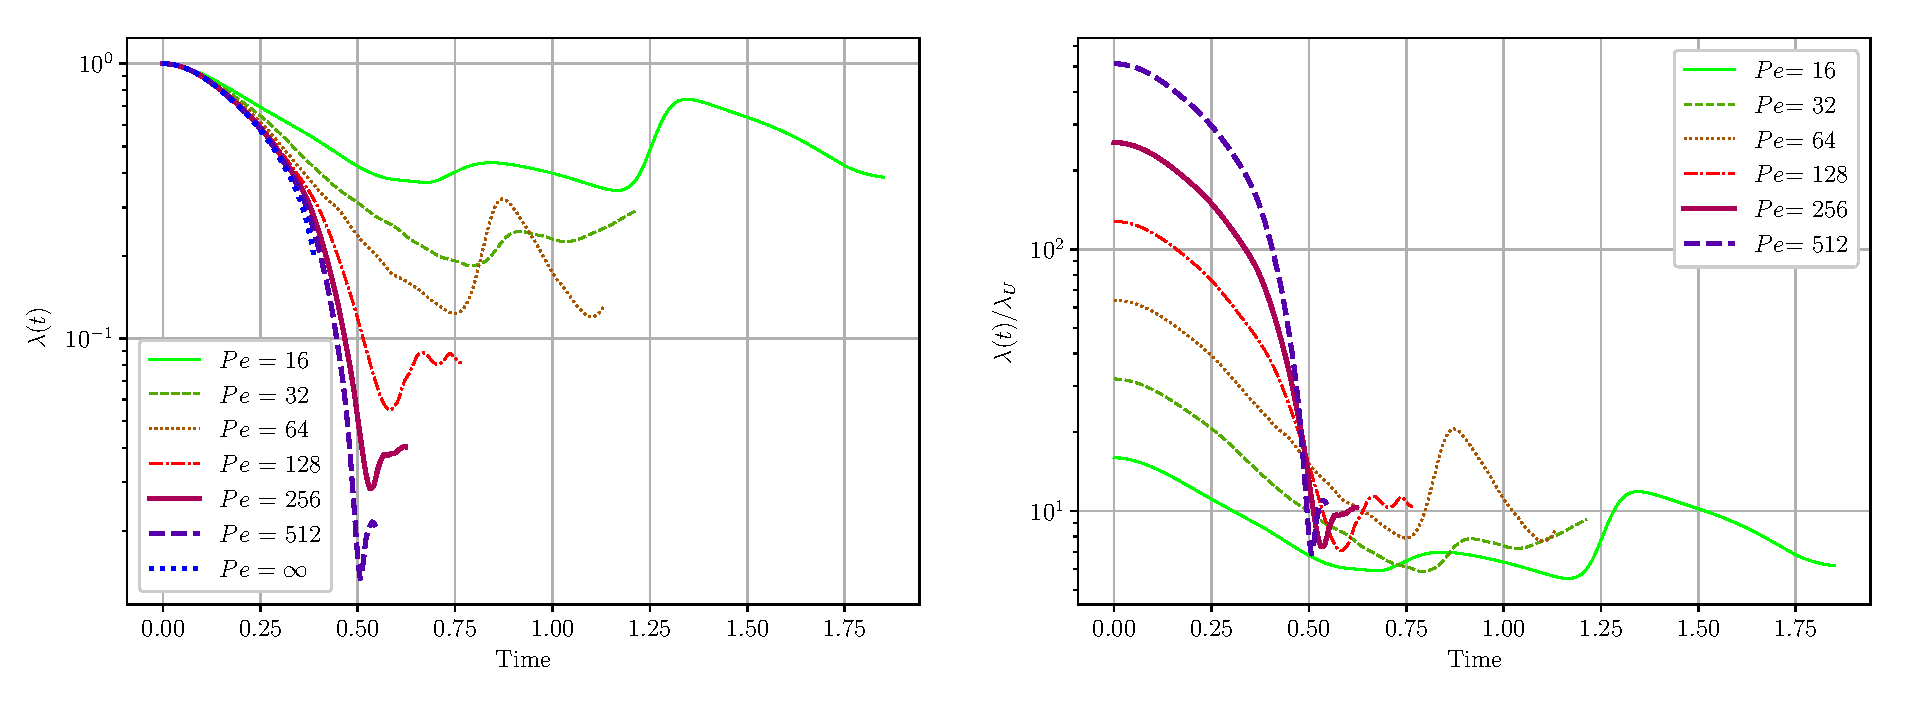
\includegraphics[width=\textwidth]{energy_length}
\caption{Energy}
\label{fig:energy_length}
\end{figure}


\begin{figure}
\centering
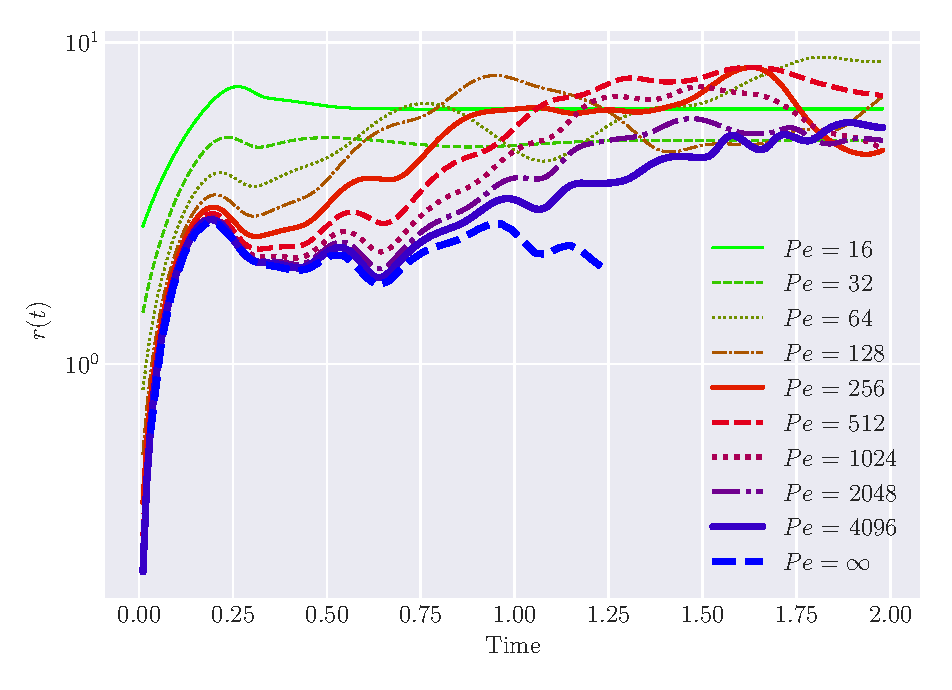
\includegraphics[width=0.5\textwidth]{enstrophy_rate}
\caption{Enstrophy}
\label{fig:enstrophy_rate}
\end{figure}



\begin{figure}
\centering
\includegraphics[width=\textwidth]{energy_rate}
\caption{Energy}
\label{fig:energy_rate}
\end{figure}



 Figure \ref{fig:enstrophy_film} shows the evolution of a scalar field under the optimal flow for the enstrophy constraint. The top film strip corresponds to $Pe =\infty$ while the bottom is $Pe = 256$. The time evolution is initially similar but soon diverges over time. Figure \ref{fig:energy_film} shows the evolution for the energy case. The top film strip corresponds to $Pe =\infty$ while the bottom is $Pe = 32$. Notice that, unlike the $Pe = \infty$ cases, the flows with finite $Pe$ are incapable of creating length scales arbitrarily small for either the energy or enstrophy cases.  The left subplot of Figures \ref{fig:enstrophy_length} and \ref{fig:energy_length} shows this phenomena more quantitatively by showing $\lambda$ over time eventually reaching a plateau. The shell-model prediction of this limiting length scale is the Batchelor scale given by $\lambda_{\Gamma} = L/\sqrt{Pe}$ for the enstrophy case and  $\lambda_{U} = L/Pe$ for the energy case. The right plots of Figures \ref{fig:enstrophy_length} and \ref{fig:energy_length} shows scaled versions of $\lambda$ given by  $\lambda/\lambda_{\Gamma}$ and $\lambda/\lambda_{U}$ respectively.  Notice how they plateau around an $O(1)$ constant. Thus, this result is consistent with the shell-model predictions. 
 
 
 Figures \ref{fig:enstrophy_rate} and \ref{fig:energy_rate} shows the rate $r$ as defined in \eqref{eq:rate}. The rate during the transient phase for the enstrophy case is $\Gamma$ which is consistent with rates expected from $Pe=\infty$ mixing studies.  For all values of $Pe$ considered, there is an increase in the rate of mixing after transient behavior has finished to a long-run rate. Surprisingly, this long-run mixing rate appears to be {\it independent} of $Pe$ for fixed enstrophy. Thus, this implies that the rate of mixing is only dependent on the rate-of-strain $\Gamma$ and not influenced by the strength of diffusion. Although, it should be noted that the onset of the long-run rate is affected by the values of $Pe$. When $Pe$ is small (strong diffusion), the Batchelor scale is reached early. From the work of \cite{GI2014} and \cite{CS2013}, $\lambda$ can decreases at most exponentially for $Pe = \infty$. If we assume that the local-in-time flows nearly saturate this bound in the transient phase, we model $\lambda$ as  $\lambda (t) = \lambda(0)\exp(- t) $ during this time. Thus, we expect the critical transition time $t_{c}$ that marks the end of this transient period is given by the condition $\lambda(t_{c})= \lambda_{\Gamma}$. Thus, this time is theorized to be $t_{c}=\ln(\lambda(0)/\lambda_{\Gamma}) = \ln ( \sqrt{Pe} )$ for $Pe>1$ (If $Pe \leq 1$, then there is no transient phase).  From the work of \cite{JMP2012} on the fixed energy case, $\lambda(t)$ can decrease linearly in time to produce perfect mixing in finite time. Thus, we model the transient phase as $\lambda(t)=\lambda(0)(1/2-t)$ where we are assuming that the optimal local-in-time flow nearly saturates the bound of the modified checkerboard flow (See Appendix \ref{appendix:checkerboard}). Therefore, we theorize that the critical transition time is $t_{c}=1/2 - \lambda_{U}/\lambda(0) = 1/2 - 1/Pe$ with $Pe> 2$ (If $Pe \leq 2$, there is not transient phase) for the energy case.
 
 
 
 For the energy case, we again have an increase in mixining rate compared to the $Pe=\infty$ transient behavior. The long-term mixing rate is proportional to $Pe$ in contrast to the long-term mixing rate of enstrophy which carried no dependence on $Pe$. 

The right subplot of Figure \ref{fig:energy_rate} is the rate $r$ divided by $Pe$. We see oscillations of $r/Pe$ around the value $1.0$ which indicates that our numerical results are consistent with our predictions from the shell model.


% Figures \ref{fig:enstrophy_norms} and \ref{fig:energy_norms} show the evolution the  $H^{-1}$,  $L^{2}$, and $H^{1}$ norms for different values of finite $Pe$.

\section{Discussion}
\label{sec:discussion}
Our local-in-time optimization results suggest that there is a limiting length scale and rate. The bounds derived under the $L^{\infty}$ constrained flow assumption did result in proving either of these observations. However, they did definitely rule out the possibility of perfect mixing in finite time in either case of enstrophy and energy. However this result may have already been known based on regularity theory of partial differential equations.  Although, we believe there is a gap between the inequalities derived. We surmise that the deficiencies in our predictions is not due to the added assumption of optimal flows belonging to $L^{\infty}$, but rather that the incompressibility condition was not fully exploited and maybe crucial to proving the limiting length scale. The analysis for energy and enstrophy constrained cases both relied on bounding the $\frac{\hone{\theta}}{\ltwo{\theta}}$ over time. This analysis allowed for the possibility of infinite growth without bound. From our local-in-time optimization analysis, we can see that this is not the case and approaches a maximum in time. Thus, we believe that this maybe a crucial step in proving the limiting length and rate. However, we have not successfully ruled out the possibility of infinite growth of this quantity over time. The the question remains, "Does there exist energy or enstrophy-constrained incompressible flows where $\frac{\hone{\theta}}{\ltwo{\theta}}$grows to infinity in time in the presence of molecular diffusion?" Or rather, can this possibility be ruled out definitively by proof.


In future work, we would like to consider the optimal control problem coined global-in-time optimization which tries to minimize the filamentation width at the end time rather than instantaneously attempting to minimize the its decay rate. This may lead to flows that are able to extend to even smaller length scales. This global-in-time optimization has been explored in the work of \cite{Miles2017a} within the context of the shell model. The authors showed that global-in-time and local-in-time optimization appeared to give similar mixing rates. 


\section{Conclusion}
\label{sec:conclusion}
We provided numerical evidence that the Batchelor scale may be the limiting scale for incompressible flows with bounded energy and enstrophy. It remains an open question if this can be proved rigorously. We also demonstrated that larger diffusion strength (larger $Pe$)  does not appear to affect the long-term mixing performance for the enstrophy case. For the energy-case, an increase in diffusion strength has an adverse affect and worsens the long-term mixing performance. .




%
%Define the spectral variance as
%%
%\begin{equation}
%		\left[ 
%			\frac{\hone{\theta}^2\hmone{\theta}^2}
%			{\ltwo{\theta}^4}  
%			- 1
%		\right].
%\end{equation}
%%
%By using this definition with H\"older's inequality provided that  $\linf{\nabla\vec{u}}\leq \Gamma$, we find that
%%
%\begin{equation}
%\label{eq:length_ineq_rate-of-strain}
%	\ddt{\lambda^2} \geq 2 1/Pe \sigma^2 - 2 \Gamma \lambda^2 .
%\end{equation}
%%
%By taking the long-time average (noted as $\langle \cdot \rangle \equiv\lim_{T\rightarrow\infty}\frac{1}{T}\int_{0}^T \,\, \cdot \,\, dt $ ) of the inequality above, we find that 
%%
%\begin{equation}
%	0 \geq  2 \kappa \tavg{\sigma^2} - 2 \Gamma \tavg{\lambda^2}.
%\end{equation}
%%
%The left hand side is zero since $\lambda^2$ is bounded by Poincar\'e's inequality. Thus, we find that
%%
%\begin{equation}
%	\tavg{\lambda^2} \geq   \lambda_{B}^2 \tavg{\sigma^2} 
%\end{equation}
%%
%where the Batchelor scale is given by $\lambda_{B} = \sqrt{\kappa/\Gamma}.$ 
%
%
%We conclude that ...
%
%By a dimensional analysis, we conjecture that the velocity field with $\hmone{\u}$=1 may be capable decreasing $\lambda$ past the Batchelor scale. 
\
\section*{Acknowledgements}

This work was supported in part by NSF Awards PHY-1205219 and DMS-1515161. One of us (CRD) is additionally grateful for Fellowship funding from the John Simon Guggenheim Memorial Foundation. We are appreciative of the valuable feedback provided by Ian Tobasco and Karen Zaya.


\appendix
\section{Mixing time of modified checkerboard flow}
\label{appendix:checkerboard}
The  consider a modified version of the checkerboard flow from \cite{JMP2012}. Suppose one starts with the initial `binary' dye concentration field where $\theta_{0}(\vec{x}) = 1$ for $x_{1}< 1/2$ and $\theta_{0}(\vec{x}) = -1$ for $x_{1}\geq 1/2$ as done in  \cite{JMP2012}. We constrain $\vec{u}$ to be  $\ltwo{\vec{u}} = 1$. 


%\section{Numerical analysis}
%\label{sec:num_analysis}
%Our conclusions rely heavily on the accuracy of our numerical solutions to the advection diffusion equations. Careful numerical analysis is thus important to make sure the length resolution is sufficient and spectral amplitudes are computed to sufficient numerical accuracy. 


\bibliographystyle{jfm}
\bibliography{manuscript}

\end{document}
